\makezhongqiinfo
\vspace{-4.4mm}\begin{longtable}{|p{156mm}|}
    \hline
    \endfirsthead
    \hline
    \endhead
    \hline
    \endfoot
    \hline
    \setlength{\parindent}{2em}
    {\bfseries研发项目进度情况:}(立项实施以来的研发工作概况;资料调研和社会调查情况;已完成的研究工作;对照原定的研究计划,如果未能按计划进行,请说明具体原因。)\par
    按照研究计划,本阶段开展了如下工作:\par
1、参考了大量中英文文献,对当前\showproject有了较为全面的了解;\par
2、完成了试验装置的设计及设备材料采购工作,并加工制作完试验装置;\par
3、以\showprojectlocation焦化废水为研究对象完成试验,开展处理工艺效果及影响因素研究,对运行参数进行调整和优化。\par \\
    \hline 
    \setlength{\parindent}{2em}
    {\bfseries已取得的阶段性成果:} \par
    经过生物滴滤池15d的稳定运行后,在温度为25-30℃,循环液pH值控制在6.5-7.0,气流量为9000m3/h的条件下,生物滤池对的氨及硫化氢的降解效果如下图。\par
{\noindent  \centering  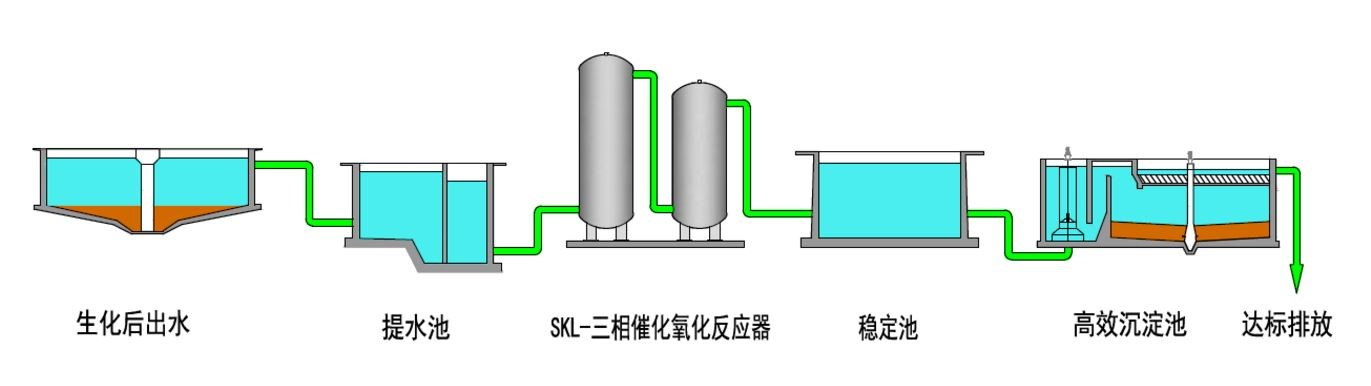
\includegraphics[width=150mm]{Img/fig1.jpg}\par}
{\hspace{40mm} 
图1 氨的进、出气浓度及去除率}
\vspace{10mm}
\par
{\noindent    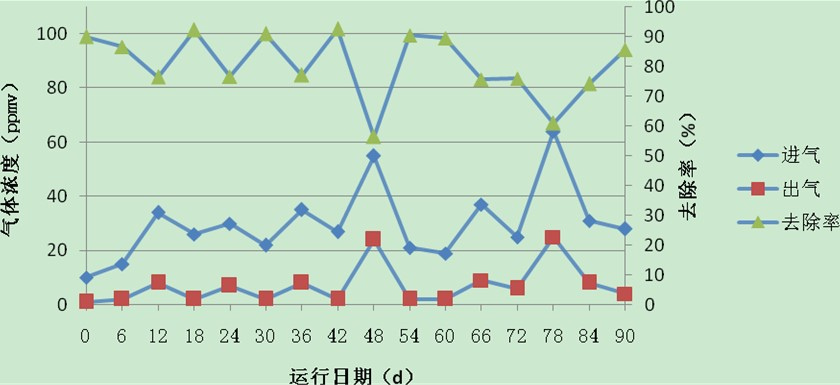
\includegraphics[width=150mm]{Img/fig2.jpg}\par}
{\hspace{40mm} 图2 硫化氢的进、出气浓度及去除率}\par
\vspace{10mm}
通过实验得出:在氨氮及硫化氢浓度在100ppmv以下,用生物滴滤池处理城市污水处理厂臭气运行效果良好。\par
 \\
    \hline 
    \setlength{\parindent}{2em}
    {\bfseries下一步研究计划和任务:} \par
    试验的结论已基本呈现,Fenton技术属\showproject中的可行技术。课题正按照计划开展,进度无延误,可进行下一步的试验研究,后续的试验工作也将按原计划及思路继续开展。具体研究计划和任务如下:\par
现在至2018年6月,设计以Fenton工艺为基础的高级催化氧化一体化设备\par
2018年6月至2018年10月,设备交付加工并运输至\showprojectlocation现场\par
2018年10月至2018年11月,在\showprojectlocation现场进行调试与数据收集分析\par
2018年11月-2018年12月,验证试验总结、项目收尾并撰写结题报告\par \\
    \hline 
    \setlength{\parindent}{2em}
    {\bfseries存在的问题、建议及其他需要说明的情况:} \par
    适合作为生物除臭工程验证的项目尚为找到。 \\
\end{longtable}

\clearpage
\begin{mdframed}[subtitlebelowline=true,subtitleaboveline=true,subtitleaboveskip=-2mm,subtitlebelowskip=5mm,subtitleinneraboveskip=1mm,subtitleinnerbelowskip=1mm]
    \mdfsubtitle{\subsection*{技术委员会意见}}
    课题研究顺利,取得成果较好,按照计划继续推进。
    \vspace*{200mm} 
    \hspace{100mm}委员会主任:\par
    \noindent\hspace{100mm}20\qquad年\quad月\quad日
\end{mdframed}